\subsection*{7.1\hspace*{0.5cm}2D Momentum - Question}
\begin{flushleft}
    A billiard ball with a mass of 0.155kg is rolling directly
    away from you at 3.5 $\frac{m}{s}$. It collides with a stationary golf ball with
    a mass of 0.05kg. The billiard ball rolls off at an angle of $15\degree$ clockwise
    from it's original direction with a velocity of $3.1\frac{m}{s}$. What is the after
    velocity of the golf ball?
\end{flushleft}
\subsection*{7.1\hspace*{0.5cm}2D Momentum - Graph and Givens}
\begin{minipage}{0.5\textwidth}
    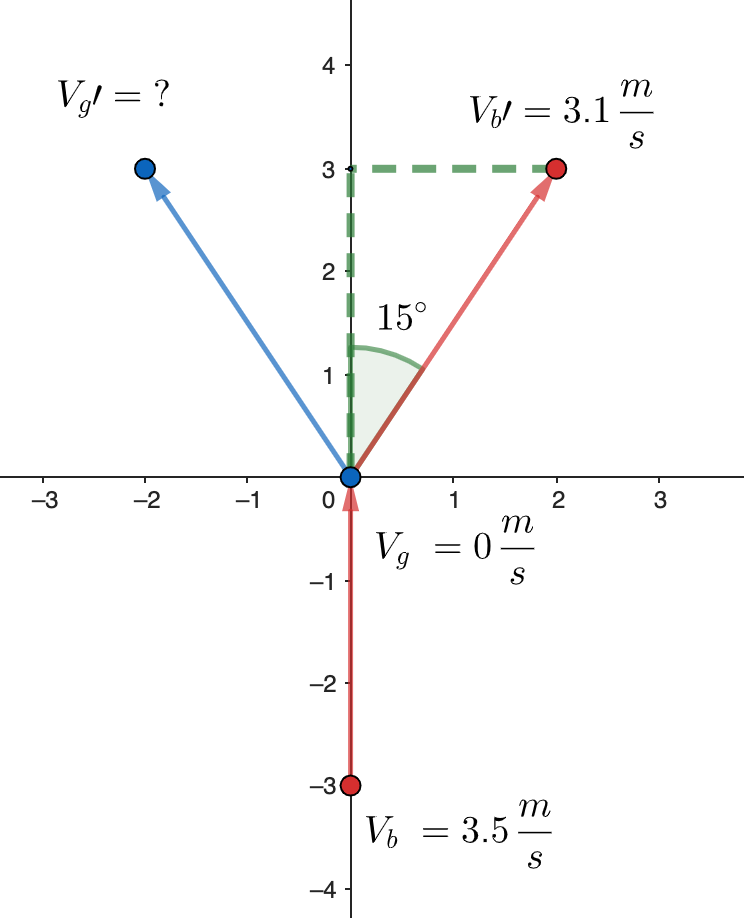
\includegraphics[scale=0.33]{./images/2d_momentum_graph}
\end{minipage}
\begin{minipage}{0.5\textwidth}
    \begin{itemize}
        \item $m_{b} = 0.155kg$
        \item $m_{g} = 0.052kg$
        \item $V_{b} = 3.5\frac{m}{s}$
        \item $V_{g} = 0\frac{m}{s}$
        \item $V_{b}\prime = 3.1\frac{m}{s}$ $[15\degree clockwise]$
        \item $V_{g}\prime = ?$
    \end{itemize}
\end{minipage}
\subsection*{7.1\hspace*{0.5cm}2D Momentum - Solve}
This solve requires both $x$ and $y$ components. Since $v_{b}$ only has a $y$ direction, $v_{b_{x}}$ is zero. Also, since $v_{g}$ isn't moving, both $v_{g_{x}}$ and $v_{g_{y}}$ are zero.\newline\newline
\textbf{1.} $P_{tot_{x}} = P_{tot_{x}}\prime$ \\
\begin{adjustwidth}{0.6cm}{0pt}
    $(m_{g})(\cancel{v}_{g_{x}}^0) + (m_{b})(\cancel{v}_{b_{x}}^0) = (m_{g})(v_{g_{x}}\prime) + (m_{b})(v_{b_{x}}\prime)$ \\\\
    $\therefore v_{g_{x}}\prime = -\left(\frac{(m_{b})(v_{b_{x}}\prime)}{m_{g}}\right) = -\left(\frac{(0.155)(3.1\sin15\degree)}{(0.052)}\right)$
\end{adjustwidth}\vspace*{15pt}
\textbf{2.} $P_{tot_{y}} = P_{tot_{y}}\prime$ \\
\begin{adjustwidth}{0.6cm}{0pt}
    $(m_{g})(\cancel{v}_{g_{y}}^0) + (m_{b})(v_{b_{y}}) = (m_{g})(v_{g_{y}}\prime) + (m_{b})(v_{b_{y}}\prime)$ \\\\
    $\therefore v_{g_{y}}\prime = \left(\frac{(m_{b})(v_{b_{y}}) - (m_{b})(v_{b_{y}}\prime)}{m_{g}}\right) = \left(\frac{(0.155)(3.5) - (0.155)(3.1\cos15\degree)}{0.052}\right)$
\end{adjustwidth}\vspace*{15pt}
\noindent\textbf{3.} Use $c^2 = a^2 + b^2$ \\
\begin{adjustwidth}{0.6cm}{0pt}
    $\therefore v_{g}\prime = \sqrt[]{{(v_{g_{x}}\prime)}^2 + {(v_{g_{y}}\prime)}^2} = \sqrt[]{{(-2.391)}^2 + {(1.507)}^2} \approx 2.766 \frac{m}{s} $
\end{adjustwidth}